\documentclass[12pt, oneside]{report}
\usepackage{IEEEtrantools}

\usepackage[margin=2.5cm]{geometry}
\linespread{1.5}
\usepackage{hyperref}
\usepackage{mathptmx}
\usepackage{xcolor}
\usepackage{hyperref}
%\usepackage[style=authoryear, defernumbers=true, backend=biber,dashed=false, maxnames=999,maxcitenames=2,giveninits=true,urldate=long,uniquename=false,uniquelist=false]{biblatex}
\usepackage[style=ieee]{biblatex}




\addbibresource{References.bib}
%\addbibresource{biblio.bib}

%% pretty captions
\usepackage{caption}
\usepackage{subcaption}
%%% allows you to create Rules, Definitions, Lemmas, Theorems etc.
\usepackage{amsthm}
\usepackage{amsmath}
\usepackage{amsfonts}
\usepackage[]{algorithm2e}

\newtheorem{theorem}{Theorem}
\newtheorem{definition}{Definition}
\newtheorem{lemma}{Lemma}
\newtheorem{Rule}{Rule}
\numberwithin{definition}{chapter}
\numberwithin{theorem}{chapter}  
\numberwithin{lemma}{chapter}  
\numberwithin{Rule}{chapter}  
\numberwithin{equation}{chapter} 
\newcommand\tab[1][1cm]{\hspace*{#1}}

 \usepackage[super]{nth} 
 
\usepackage{graphicx}
\usepackage{wrapfig}
\usepackage{placeins}
\usepackage{pdfpages}
\usepackage{attachfile2}

\usepackage[utf8]{inputenc}
\usepackage[T1]{fontenc}
\usepackage{csquotes}

\usepackage{fancyhdr}
%\pagestyle{fancy}
\renewcommand{\headrulewidth}{0.4pt}
%\renewcommand{\footrulewidth}{0.4pt}
\fancyhead{}
\fancyhead[L]{SHORTENED TITLE} %%% CHANGE AS APPROPRIATE (you may need to use a shortened form of the title)
\fancyhead[R]{Student ID: .......} %%% CHANGE AS APPROPRIATE
\fancyfoot{}
\fancyfoot[C]{\thepage}

\usepackage{titlesec}
\titlespacing{\chapter}{0pt}{*4}{*2.5}

\titleformat{\chapter}{\normalfont\huge\bf}{\thechapter}{20pt}{\huge\bf}
%% prevents Chapter 1 (then new line and Introduction) - turns into 1. Introduction


%% Call your references "References" rather than Bibliography, then also allow for a separate Bibliography if needed.

\DeclareSourcemap{
  \maps[datatype=bibtex]{
    \map{
      \perdatasource{references.bib}
      \step[fieldset=keywords, fieldvalue={, primary}, append]
    }
    \map{
      \perdatasource{biblio.bib}
      \step[fieldset=keywords, fieldvalue={, secondary}, append]
    }
  }
}
%%%%%%%%%%%%%%%%%%%%%%%%%%%%%%%%
%  Don't make any changes here
%  This defines formatting style
%%%%%%%%%%%%%%%%%%%%%%%%%%%%%%%%

\DeclareNameAlias{sortname}{last-first}
\DeclareFieldFormat{edition}{%
  \ifinteger{#1}
    {\ifnumequal{#1}{1}%
     {}%
     {\mkbibordedition{#1}~\bibstring{edition}}%
    }
    {#1\isdot}}

\DeclareFieldFormat[article,inbook,incollection]{title}{#1\isdot}
\DeclareFieldFormat[article,inbook,incollection]{citetitle}{#1\isdot}

\newrobustcmd{\MakeTitleCase}[1]{%
  \ifboolexpr{test {\ifentrytype{article}} or test {\ifentrytype{inbook}} or test {\ifentrytype{incollection}}}
    {#1}
    {\MakeSentenceCase{#1}}}

\DeclareFieldFormat{urldate}{\bibsentence\mkbibbrackets{\bibstring{urlseen}\space#1}}
\DeclareFieldFormat{url}{\bibstring{urlfrom}\addcolon\space\url{#1}}

\renewbibmacro*{journal}{%
  \iffieldundef{journaltitle}
    {}
    {\printtext[journaltitle]{%
       \printfield[titlecase]{journaltitle}%
       \setunit{\subtitlepunct}%
       \printfield[titlecase]{journalsubtitle}}
       \ifboolexpr{
         not test {\iffieldundef{url}}
         or
         not test {\iffieldundef{urldate}}
         or
         not test {\iffieldundef{doi}}
         or
         not test {\iffieldundef{eprint}}
       }
         {\nopunct\bibstring[\mkbibbrackets]{online}}%
         {}}}

\renewbibmacro*{journal+issuetitle}{%
  \usebibmacro{journal}%
  \setunit*{\addspace}%
  \iffieldundef{series}
    {}
    {\newunit
     \printfield{series}%
     \setunit{\addspace}}%
  \newunit
  \usebibmacro{volume+number+eid}%
  \setunit{\addspace}%
  \usebibmacro{issue+date}%
  \setunit{\addcolon\space}%
  \usebibmacro{issue}%
  \newunit}

\NewBibliographyString{online}
\DefineBibliographyStrings{english}{%
  urlseen    = {accessed},
  online     = {online},
}
%\addbibresource{example.bib}
\renewcommand*{\nameyeardelim}{\addcomma\addspace}
\renewbibmacro{in:}{%
  \ifentrytype{article}{}{\printtext{\bibstring{in}\intitlepunct}}} % removes "In" preceeding journal title
\setcounter{tocdepth}{1} % allow only sections (not subsections in table of contents)

\begin{document}
\begin{titlepage}
    \begin{center}
        \vspace*{1cm}
        {\huge
        INSERT TITLE HERE }
        \vspace{0.5cm}
        \\
        {\large By}
        \\
        \vspace{0.5cm}
        \textbf{SURNAME(S), FORENAME(S)}
   		\vspace{1.5cm}
        \center{\huge{\textbf{MSc Robotics Dissertation}}}
        \\
        \vspace{0.25cm}
       
\includegraphics[scale=0.6]{logos/bristolcrest_colour.pdf}
        \hspace{5mm}
        
\includegraphics[scale=0.35]{logos/UWE_insignia.png}

        \vspace{10mm}
        {\large Department of Engineering Mathematics\\
        \textsc{University of Bristol}}
        \\
        \&
        \\
        {\large Department of Engineering Design and Mathematics\\
        \textsc{University of the West of England}}\\

        \vspace{0.8cm}
        \begin{minipage}{10cm}
        \center A MSc dissertation submitted to the University of Bristol and the University of the West of England in accordance with the requirements of the degree of \textsc{Master of Science in Robotics} in the Faculty of Engineering.
        \end{minipage}\\
        \vspace{0.8cm}
        \today
        
    \end{center}
    
 

\end{titlepage}
\chapter*{Declaration of own work}

I declare that the work in this MSc dissertation was carried out in accordance with the requirements of  the University's Regulations and Code of Practice for Research Degree Programmes and that it  has not been submitted for any other academic award. Except where indicated by specific  reference in the text, the work is the candidate's own work. Work done in collaboration with, or with the assistance of, others, is indicated as such. Any views expressed in the dissertation are those of the author.


 \begin{flushright}
 
 Name and Date
\end{flushright}

\newpage
\chapter*{Acknowledgement}
% Add here text if you would like to thank somebody, e.g., your family, friends, colleagues, supervisors, etc.

I would like to thank ... 


\chapter*{Abstract}
\textbf{
Abstract should give a short summary of the motivation, the approach and important insights and results.}
%
\vfill
\begin{flushright}
 Number of words in the dissertation: .... words.
\end{flushright}
    
 %% any other "Front matter" should go here before the table of contents - format in a style similar to the file Abstract.tex
\tableofcontents 
\listoftables
\addtocontents{toc}{~\hfill\textbf{Page}\par} % comment this line out if you want to remove "Page"
%%%%%%%%%%%%%%%%%%%%%%%%%%%%%%%%%%%%
\chapter{Introduction}
\label{chap:Introduction}
%%%%%%%%%%%%%%%%%%%%%%%%%%%%%%%%%%%%
The introduction should provide:
\begin{itemize}
    \item A clear explanation of the problem that you tackle
    \item Motivation why this is interesting and worth investigating
\end{itemize}

To improve communication, it is also recommended that you concisely state the aims and objectives of your project.  As part of the introduction, these can be generally stated and not require specialist knowledge.  Use the next chapter "Literature Review" to provide specialist knowledge for the reader.
\begin{enumerate}
    \item \textbf{Aims:} The aims of a project are \emph{what you hope to learn}.
        \begin{enumerate}
        \item "To understand why X varies with Y..."
        \item "To evaluate [technology] when exposed to unexpected conditions so that..."
        \item "To increase understanding of ..."
        \item \emph{etc...}
        \end{enumerate}
    \item \textbf{Objectives:} The objectives are \emph{the elements which are necessary to conduct the project}.
        \begin{enumerate}
            \item "To properly design an experiment methodology to mitigate...."
            \item "To construct a robotic system including ... to collect meaningful data."
            \item "A complete analysis of ... must be conducted prior to the full system evaluation in order to..."
            \item \emph{etc...}
        \end{enumerate}
\end{enumerate}

You can then repeat and address these explicitly in your Conclusion when evaluating the success and challenges of your project. 
    



% standard chapter format
%%%%%%%%%%%%%%%%%%%%%%%%%%%%%%%%%%%%
\chapter{Literature Review} 
\label{chap:Literature_Review}
%%%%%%%%%%%%%%%%%%%%%%%%%%%%%%%%%%%%

Use your literature review to help the reader to understand the value and the interest in your project.  You should look for related works already published that either support the merit of your project, or provide the background understanding/information to make your new claims.  Try to avoid writing a "catalogue" of related works (e.g this would have little of your own insight added).  Instead, describe to the reader why the related work is interesting or relevant to your own work.  What did they achieve?  What did they overlook?  It is highly recommend you finish your Literature Review with a final subsection "Summary", where you may wish to formulate highly specified research questions or hypotheses, or assert the need for your Research Methodology (next chapter).  

introduction
literature review
implementation
research methodology
results




\section{This is a section}
\subsection{This is a subsection}
\subsubsection{This is subsubsection}

%%%%%%%%%%%%%%%%%%%%%%%%%%%%%%%%%%%%
% Figure with subfigures
%%%%%%%%%%%%%%%%%%%%%%%%%%%%%%%%%%%%

\begin{figure}[htb]
\centering
\begin{subfigure}[t]{.5\textwidth}
  \centering
  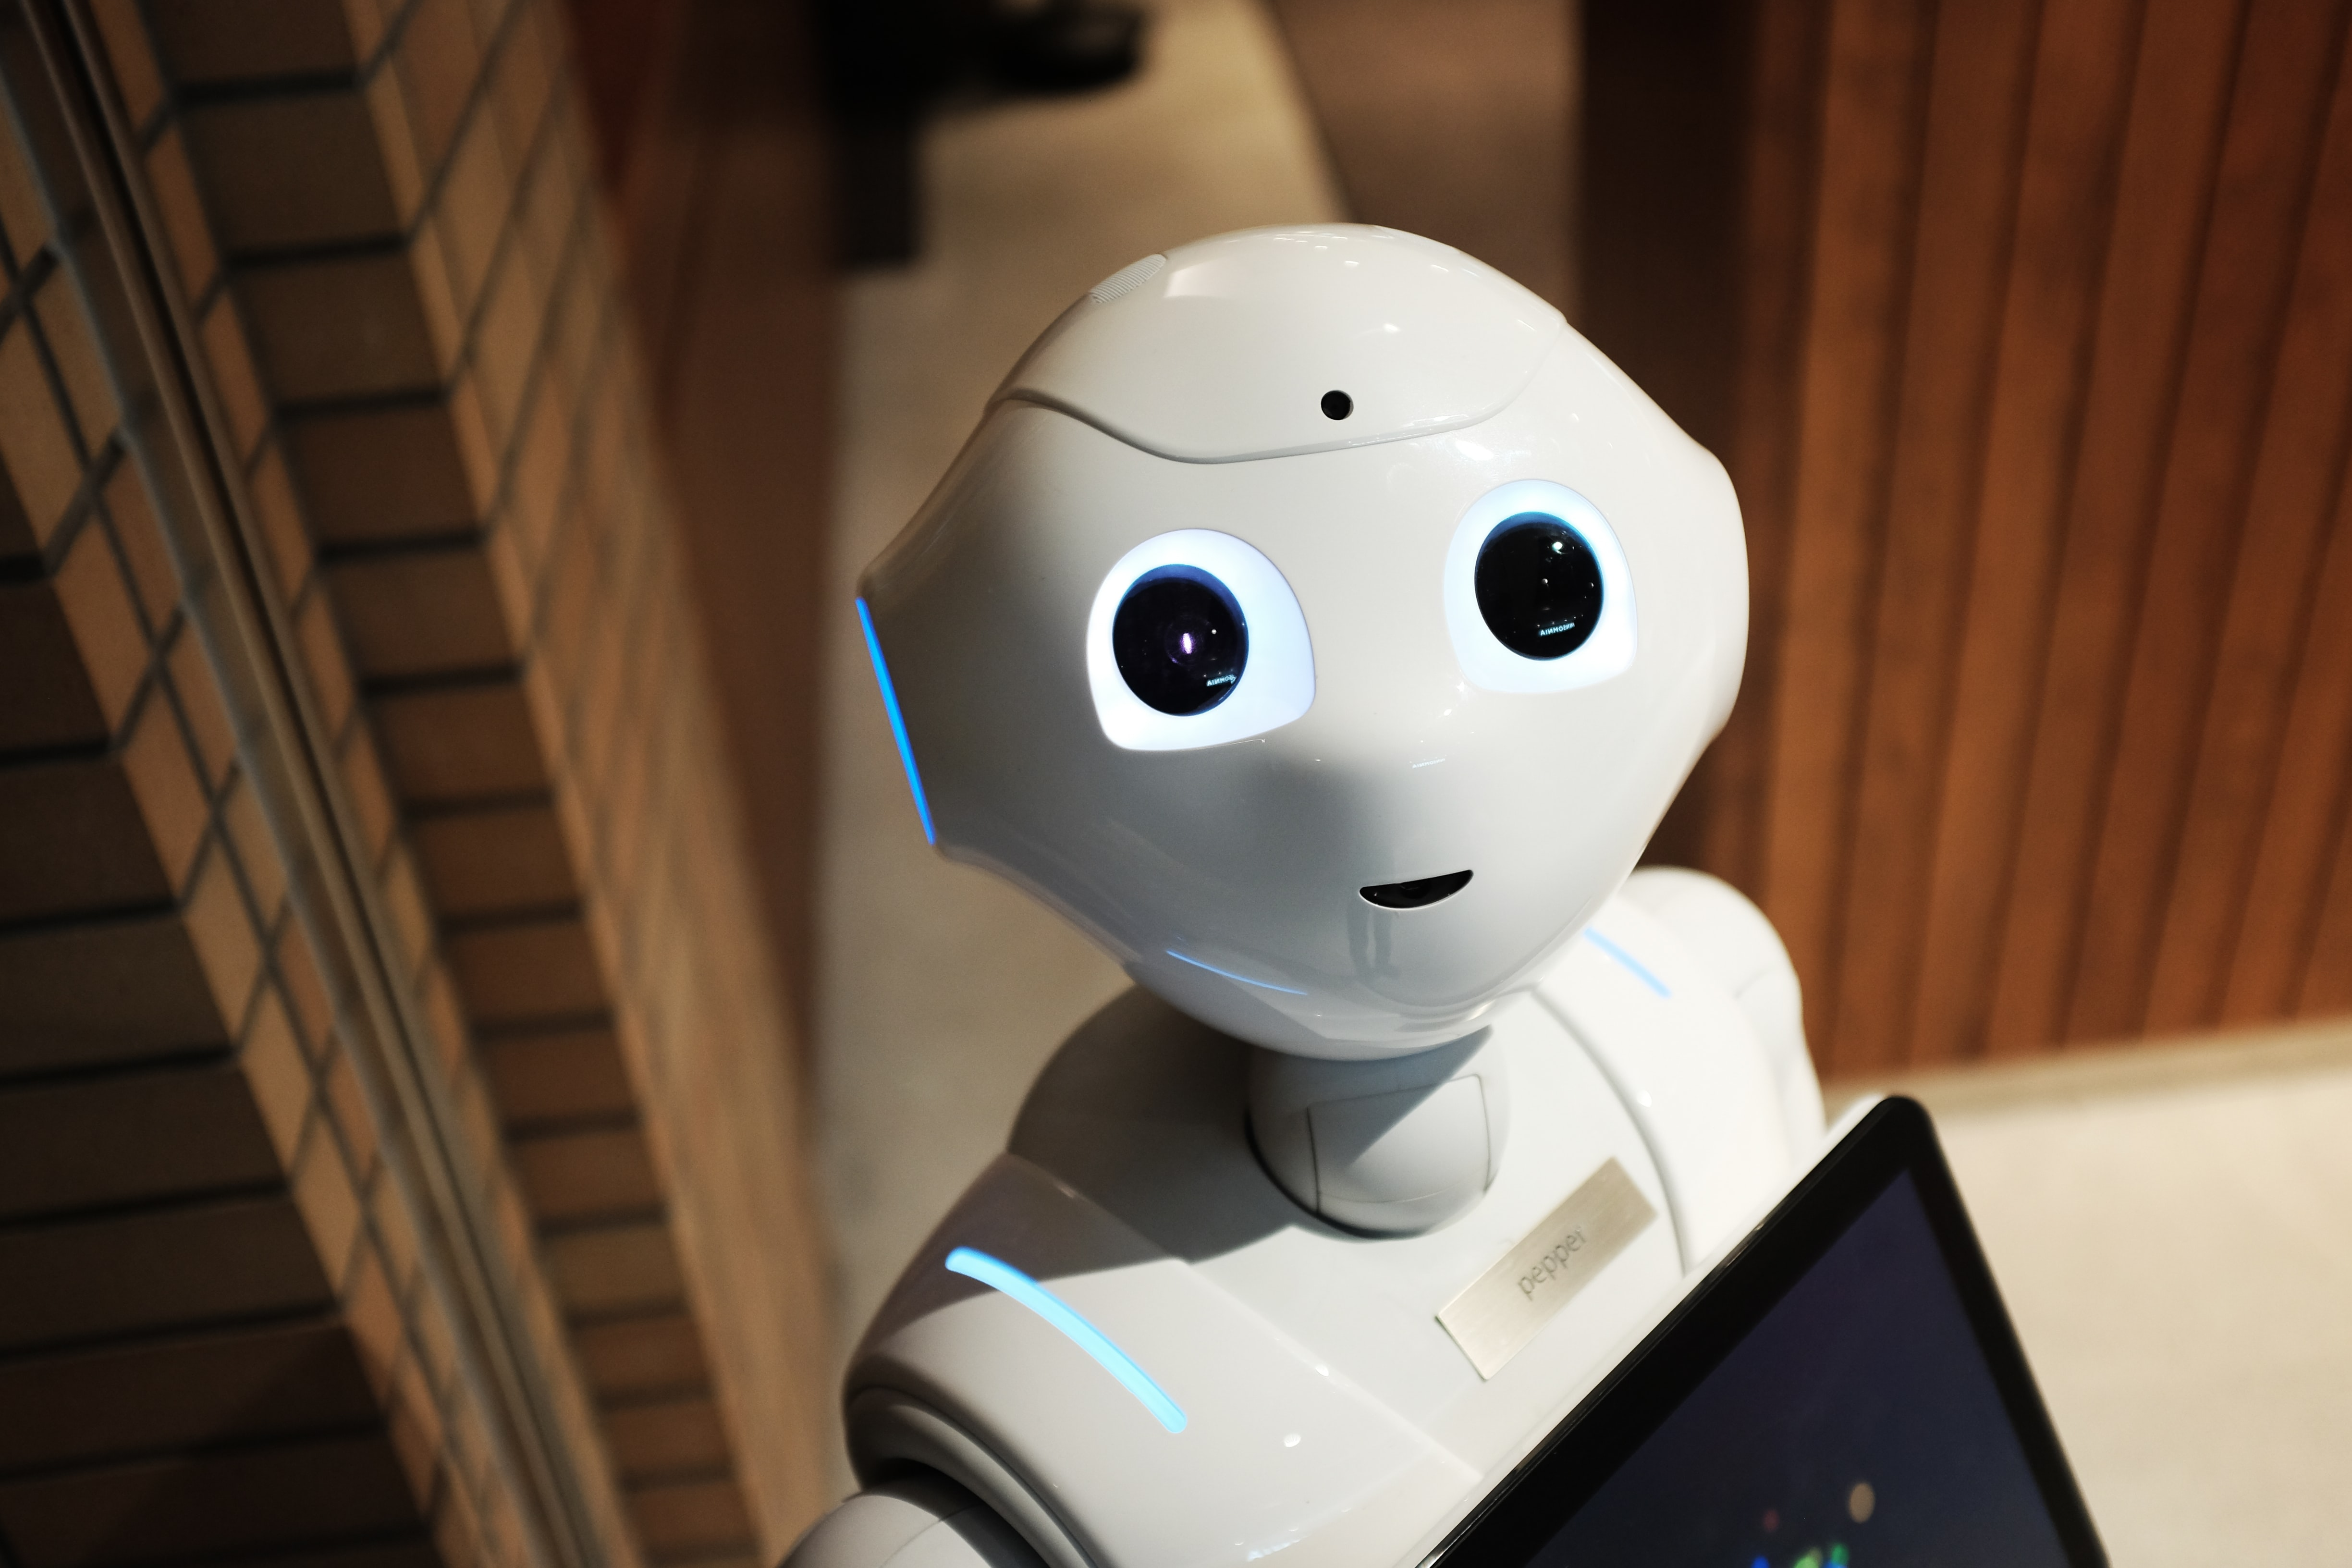
\includegraphics[height=4.5cm]{figures/Robot_1.jpg}
  \caption{\label{fig:left_robot} This is a robot.}
  \label{fig:theoretical}
\end{subfigure}%
\begin{subfigure}[t]{.5\textwidth}
  \centering
  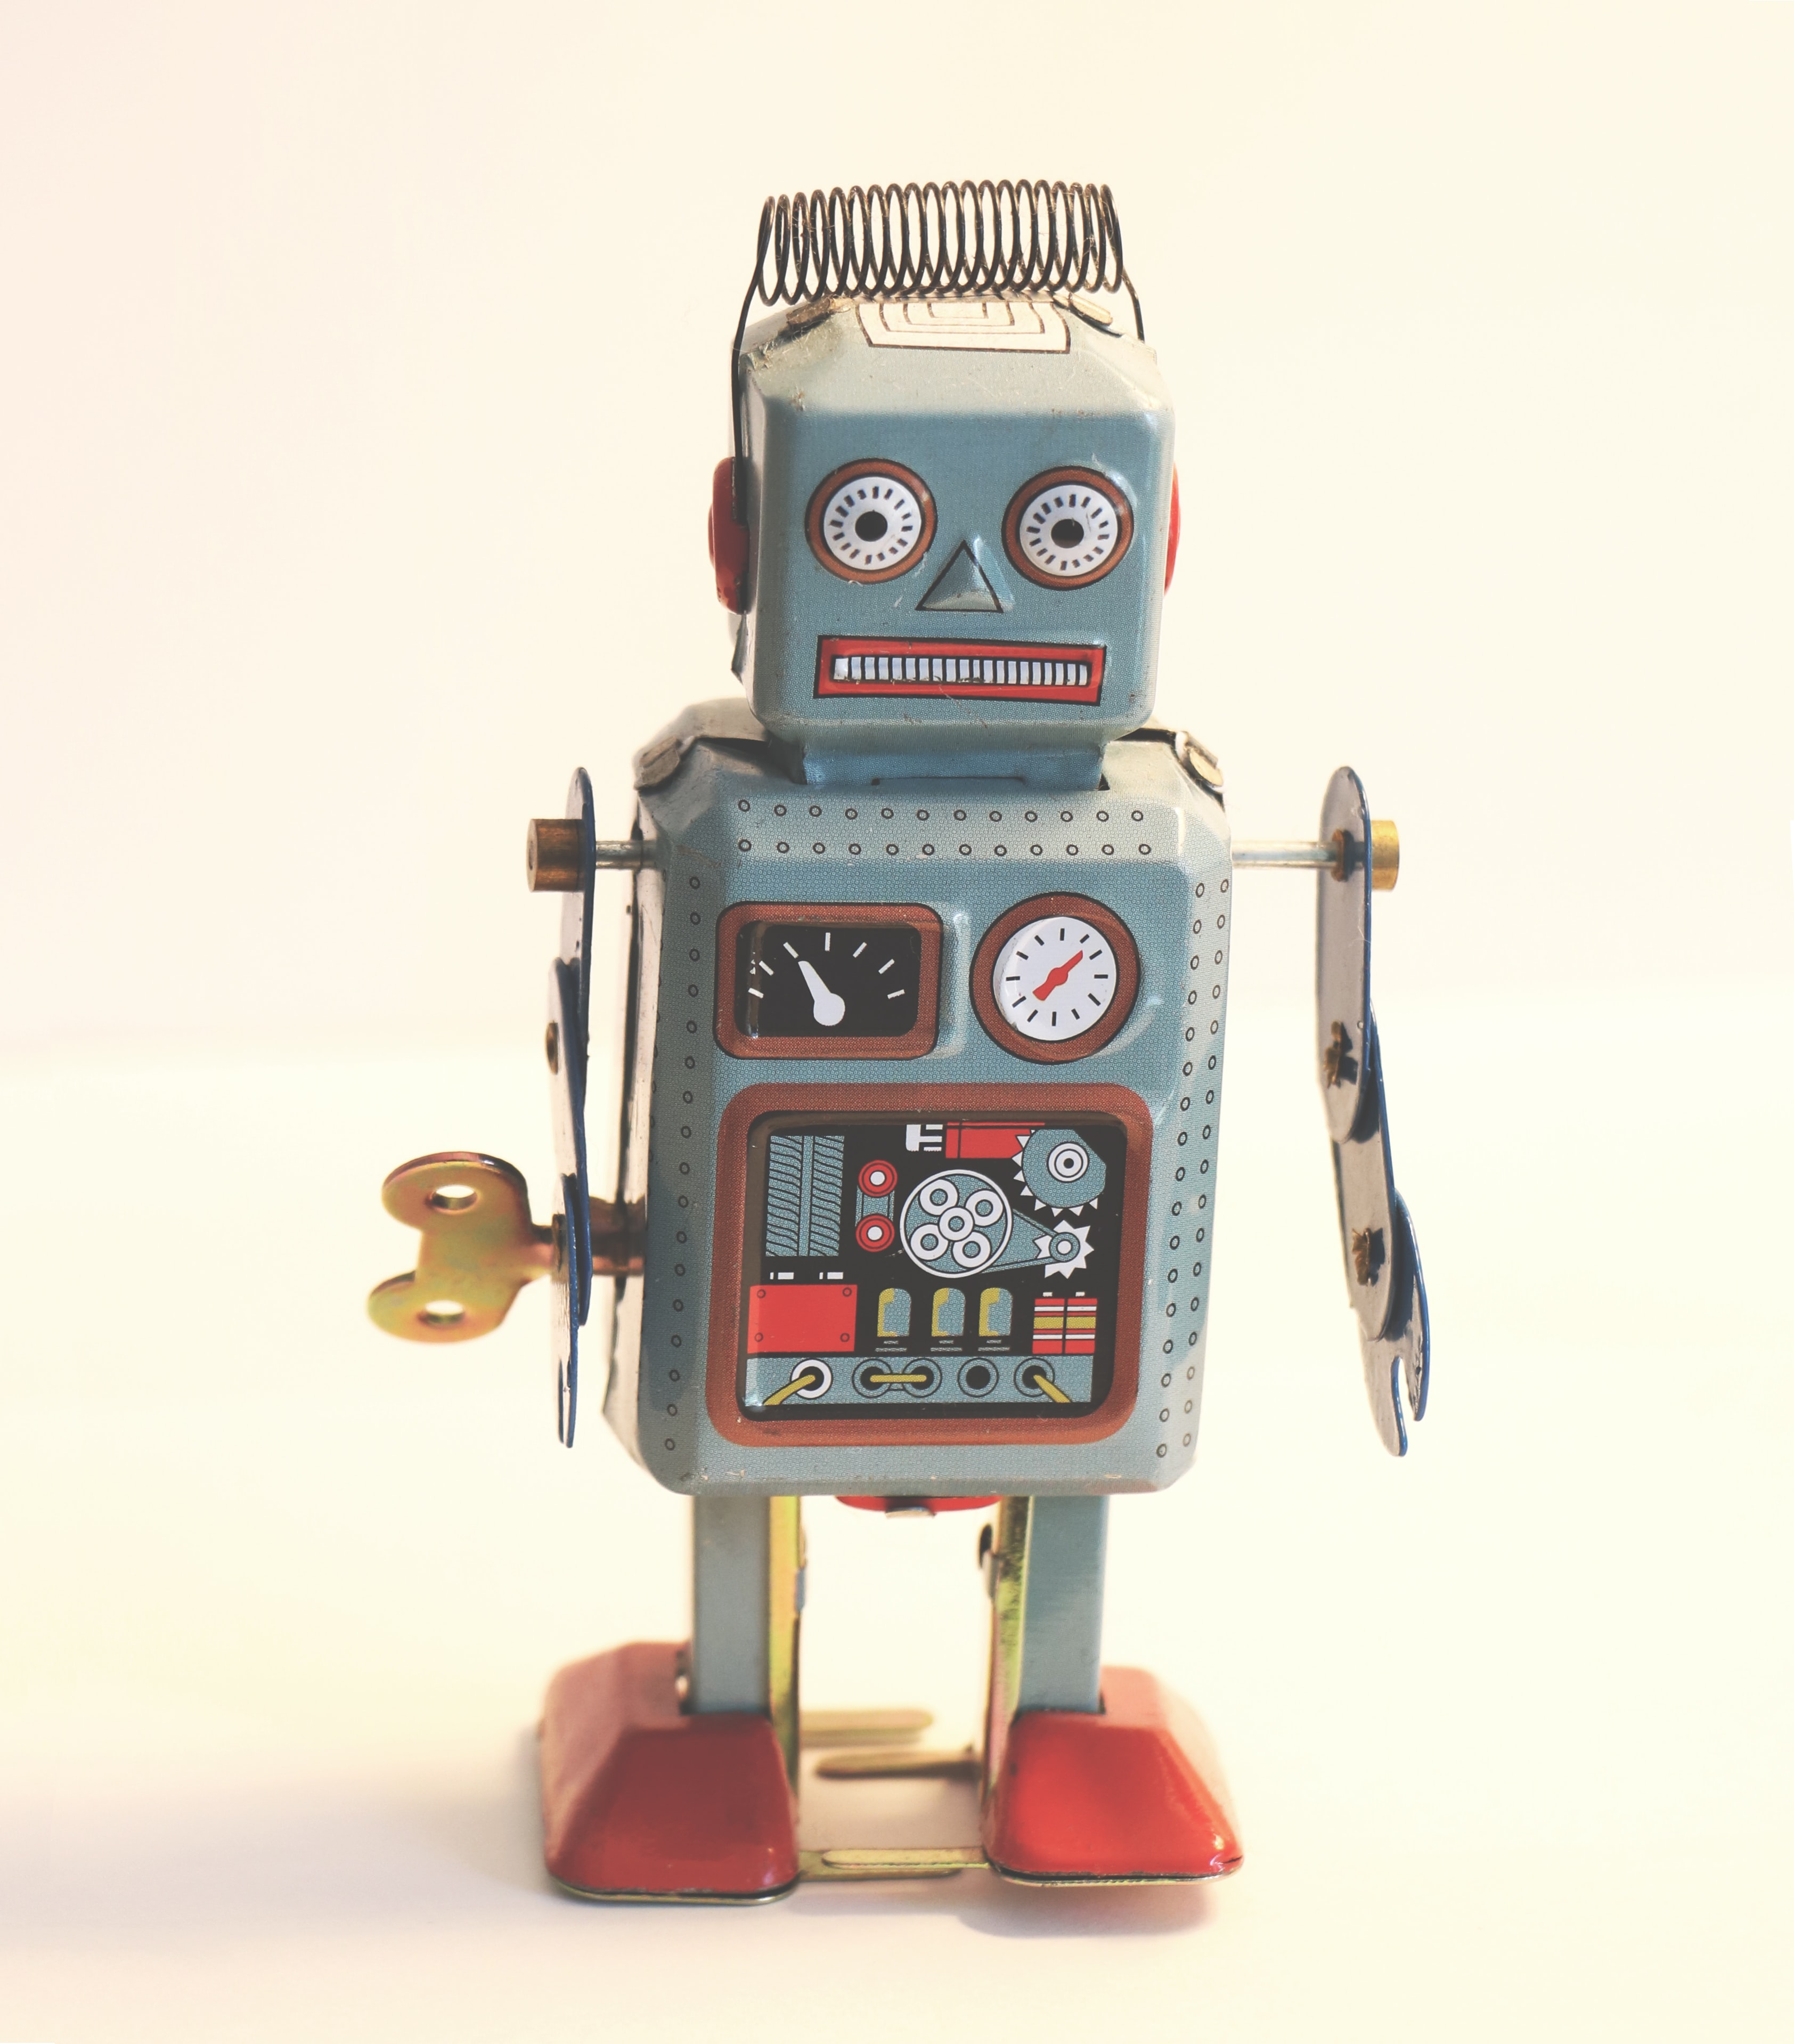
\includegraphics[height=4.5cm]{figures/Robot_2.jpg}
  \caption{\label{fig:right_robot} This another robot.}
  \label{fig:practical}
\end{subfigure}
\caption{\label{fig:two_robots} These are two robots}
\label{fig:test}
\end{figure}

For example, \cite{Robots2020} discusses the two robots depicted in Figure \ref{fig:two_robots}. There is a robot in Figure \ref{fig:left_robot} and another robot in Figure \ref{fig:right_robot}.



%%%%%%%%%%%%%%%%%%%%%%%%%%%%%%%%%%%%
\chapter{Research Methodology}
\label{chap:Literature_Review}
%%%%%%%%%%%%%%%%%%%%%%%%%%%%%%%%%%%%
The Methodology section should provide a clear explanation of the research approach.  You want your reader to agree that you carefully considered your method so that we can trust your results to be both insightful (\underline{mean something}) and credible (\underline{not subject to error}):
\begin{itemize}
    \item A clear description of the methodology, how it creates a scientific investigation and operates to collect meaningful data.
    \item A clear justification of \underline{why} you have chosen this particular approach.
    \item Information needed for a reader to understand \underline{how} you did it (can a reader \underline{reproduce} your work, and collect equally valid results? e.g. hardware/software used, configuration, number of trials, any procedures used, etc.)
    \item A description of any approaches taken to process collected data, e.g. metrics are used to combine data in a meaningful way - you should state any used explicitly, their utility, their suitability to your methodology and their limitations.  
\end{itemize}



As on can see in Table \ref{tab:Table_with_numbers} there are numbers involved. 

%%%%%%%%%%%%%%%%%%%%%%%%%%%%%%%%%%%%
% If you have more complex tables you can 
% get a corresponding LaTeX code here
% https://www.tablesgenerator.com 
%%%%%%%%%%%%%%%%%%%%%%%%%%%%%%%%%%%%
\begin{table}[h!]
\centering
 \begin{tabular}{|c | c | c | c|} 
 \hline
  Frame number & User 1 state & User 2 state & Resulting state \\ [0.5ex] 
 \hline
 \hline
  n & 0 & 0 & 1 \\ 
 \hline
  n+1 & 0 & 1 & 2\\
 \hline
  n+2 & 1 & 0 & 3 \\
 \hline
  n+3 & 1 & 1 & 4 \\
 \hline
\end{tabular}
\caption{\label{tab:Table_with_numbers}An example of a table.}
\label{table:example}
\end{table}

For example, if $x>0$ then we can write
\begin{equation}
\label{eq:sum}
\sigma =\int_{x=0}^{\infty} \frac{1}{x^2}dx \quad ,
\end{equation}
where $\sigma$ is the integral (see Equations \ref{eq:sum}).  



%%%%%%%%%%%%%%%%%%%%%%%%%%%%%%%%%%%%
\chapter{Results}
\label{chap:Results}
%%%%%%%%%%%%%%%%%%%%%%%%%%%%%%%%%%%%
The Results section should provide
\begin{itemize}
    \item An overview of all obtained results
    \item An in detail discussion/explanation of all results
    \item A scientific interpretation of the results
\end{itemize}


\section{Common attributes to pay attention to are:}
\begin{itemize}
    \item When comparing plots, keep the scale of axes consistent.  To do otherwise is misleading for the reader.
    \item If you are going to compare separate plots, consider if they can be better evaluated when combined into a single plot.
    \item When plotting data, particularly the \emph{mean}, ensure that you also plot error bars (or other method) of indicating the distribution.
    \item If a figure or plot is included, ensure it is referenced explicitly in the body text discussion.
    \item When a large table of data is included, consider whether it would be better communicated as a box-plot or something similar.
    \item All axes should be labelled and include units of measurement where applicable.
    \item All captions and figures should have captions with enough information to be understood at a glance.  Do not use captions to provide information that is better placed in the body text.  
    \item Remember to identify result outliers and anomalous data and to attempt an explanation or justification.
\end{itemize}

\
\chapter{Discussion and Conclusion}
% please replace this text with your own
The conclusion needs to provide
\begin{itemize}
    \item A short summary (What has been done and what are the main results)
    \item Limitations of your work, where applicable. 
    \item Discussion of your work in the bigger picture (How does this contribute to the research field?)
    \item Future work (What could be next steps in this work?).  Remember to keep future work realistic.  A good approach is to discuss what the next progression of this project would be, and to justify why this would be interesting.  
\end{itemize}

You will find it easier to write your conclusion if you copy-and-paste your \emph{Aims, Objectives}, and any research questions or hypotheses you stated.  You can then discuss each of these explicitly in turn, and how you were able to answer them or complete them successfully.  When things have not gone as well as you would have hoped, demonstrate your critical thinking and reasoning to analyse the short-comings of your project - to demonstrate that you understand the underlying causes and that you could conduct good futurework from this learning experience.  
\vfill



%%%%%%%%%%%%%%%%%%
\appendix
\input{appendix}  % uncomment  these two lines of code if you have don't have an appendix!

\printbibliography[ title= References]\addcontentsline{toc}{chapter}{References}


\end{document}
